
\chapter{Općenito o ExRec-u}
U radu \citep{exrec} prepoznata je neefikanost prevladavajućih sustava otvorenih online tečajeva (MOOC) zbog dodjeljivanja istih vježbi svim studentima. S druge strane, personalizirani sustavi preporuka zadataka mogu poboljšati efikasnost učenja prilagođavajući se razini znanja svakog studenta (učenika, korisnika). Takvo razmišljanje uvelike odgovara našem problemu. U originalnom radu krenulo se od temeljne pretpostavke da je ubrzavanje učenja temeljni cilj svakog personaliziranog sustava preporuke zadataka u obrazovanju. Rad predlaže personalizirani sustav preporuke zadataka za online učenje poboljšanjem performansi postojećih \textit{knowledge tracing} modela. Napominje se da postojeći modeli praćenja znanja ne koriste informacije o pripadnosti zadataka konceptima. Konkretno, ovim radom modificira se \textit{dynamic key-value memory network knowledge tracing (DKVMN)} model tako da se memorijska struktura temelji na listi koncepata određenog tečaja eksplicitno bilježeći vezu zadataka i koncepata tijekom procesa praćenja znanja. Model je korišten za izgradnju simulatora studenata korištenog za treniranje strategije preporuke zadataka pomoću podržanog učenja. \newline
\newline
\section{Povezani radovi} %višak? %citate dodati na početna poglavlja ukupnog doca
ExRec je sustav sastavljen od praćenja znanja i preporuke zadataka. Nadogradnja je već poznatih i istraženih sustava. Praćenje znanja inače često koristi prije istražen i implementiran Bayesovski model praćenja znanja (BKT). Modelira studentovo znanje koncepta kao binarnu varijablu i, koristeći skriveni Markovljev model, ažurira vjerojatnost njegova ovladavanja konceptom uzimajući u obzir rezultate rješavanja zadataka. Taj je model na razini koncepata i zanemaruje odnose između različitih koncepata.\newline
Drugi pristup može se pronaći u također već istraženom modelu dubokog praćenja znanja (DKT) s povratnom neuronskom mrežom. Modelira znanje studenta kao latentnu varijablu. DKT je korišten i za sustav preporuke.\newline
\newline
Preporuke zadataka većinom koriste heurističke algoritme. Studentu se preporučuje zadatak ako je vjerojatnost da će ga točno riješiti oko 50\%. Optimalnost takvog algoritma je upitna.\newline
Koristi se i pristup određivanja ZPD-a (zona proksimalnog razvoja, engl. \textit{Zone of Proximal Development}) na temelju trenutnog znanja učenika, a zatim se odabire najkorisniji zadatak pomoću algoritma više naoružanih razbojnika (engl.\textit{ multi-armed bandits algorithm}).\newline
SPARFA framework se koristi za procjenu znanja svakog učenika iz njihovih prethodnih rezultata. Zatim koristi te profile znanja kao kontekst i primjenjuje kontekstualni algoritam naoružanih razbojnika za preporuku zadataka kako bi se maksimizirao učenikov neposredan uspjeh, odnosno njegov uspjeh na sljedećem zadatku. Problem ovog algoritma je što uzima u obzir samo sljedeći korak (kratkoročna nagrada) stoga njegova izvedba ne mora biti optimalna.\newline
\newline
\section{Pozadina sustava i dataset}
Originalni ExRec sustav kao dataset uzima uzorke studentskih interakcija iz IPS-a (engl. \textit{Intelligent practice System}.
IPS je kineski online sustav za samostalno učenje. U IPS-u svaki tečaj ima na desetke gradiva, a student sam bira željeno gradivo. Svako gradivo ima 7 stadija iz kojeg je moguće izaći u bilo kojem trenutku (ili promijeniti gradivo):
\begin{enumerate}
\item vježbe za zagrijavanje prije nastave
\item vježbe na nastavi prije predavanja
\item video predavanja
\item vježbe na nastavi nakon predavanja
\item domaća zadaća
\item vježbe pregleda gradiva
\item vježbe pregleda raznih gradiva.
\end{enumerate}
Svaka vježba (zadatak) ima tri hijerarhijske oznake koncepata (\textit{tagove}) koje su im pridijelili eksperti. U stadijima od 1 do 5 uključeni su sadržaji jednog koncepta, dok 6 i 7 sadrže vježbe drugih koncepata zbog procjene naučenosti. Sustav sprema trajanje studentovog učenja u svakom stadiju, vježbe koje polaže i točnost rezultata.\newline
\newline
Za potrebe našeg projekta napravljena je skripta koja pretvara Assistments dataset (skillbuilder.csv) u format potreban za generiranje preporuka.\newline
Za svakog studenta rezervirana su 4 retka:
\begin{itemize}
\item[-]prvi redak je broj odgovorenih pitanja/vježbi,
\item[-]drugi redak je lista identifikacijskih brojeva pitanja,
\item[-]treći redak redoslijed točnosti odgovora na pitanja, a
\item[-]četvrti redak sadrži koncept prve razine svakog pitanja.
\end{itemize}
\section{DKVMN - model za praćenje znanja}
DKVMN se generalno sastoji od statičke matrice (ključa) koji sprema latentne koncepte i dinamičke matrice (vrijednosti) koja sadrži razine savladnosti određenog koncepta. Model računa korelaciju vježbe i latentnog koncepta u ključu. Korelaciju koristi za čitanje studentovih razina savladanost koncepta i predviđa točnost ishoda rješavanja zadatka.\newline
\subsection{Concept Aware struktura}
DKVMN ExRec praćenja znanja poboljšan u aspektima memorijske strukture, težina koncepata znanja te procesa pisanja i čitanja. Osnovni DKVMN dizajn je modificiran tako da memorijska struktura ovisi o listi koncepata nekog tečaja. Na slici
<> je prikazana struktura modela. $M^k_t$ je matrica ugrađenih koncepata veličine $M X N$ gdje je $N$ broj memorijskih lokacija, a $M$ je veličina vektora na svakoj lokaciji. $N$ se postavlja na broj koncepata znanja određenog tečaja. Pošto se u radu koristilo 1 koncept prve razine, 7 koncepata druge razine te 15 treće razine N=23. Nakon toga, na svakoj lokaciji koncepta znanja se sprema studentovo znanje.


	\begin{figure}[!htb]
	\centering
	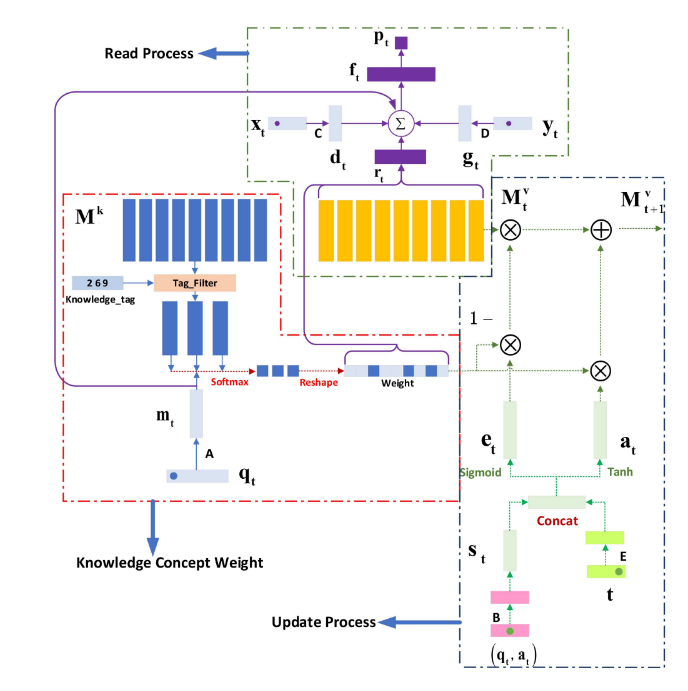
\includegraphics[scale=0.8]{exrec1.png}
	\caption{}
	\label{}
\end{figure}


\subsection{Knowledge Concept Weight}

Pošto je studentovo stanje koncepta znanja spremljeno u memoriji, kada se pojavi novi zadatak dohvaćaju se i osvježavaju samo memorijske lokacije povezane s tom vježbom. Za svaki koncept znanja se računa težina, težine se koriste kako bi se izračunala težinska suma trenutnih stanja koncepata znanja korisnika kako bi se predvidio njegov rezultat na vježbi. Također će se koristiti kako bi se osvježio korisnikovo stanje znanja nakon primitka rezultata od zadatka.

Prvo se dohvaćaju ugrađene vrijednosti od danog zadatka. Kao što se vidi na slici kada zadatak $q_t$ dođe u trenutku $t$ prvo se transformira u ugrađeni vektor $m_t$ kroz ugrađujuću matricu $A$, tada se KCW računa pomoću algoritma 1. Ukratko, DKVMN računa težinske veze između zadataka i skrivenih koncepata znanja, dok se u ovom kodu računaju samo veze između zadataka i poznatih povezanih koncepata, nepovezani koncepti se postavljaju na 0.


	\begin{figure}[!htb]
	\centering
	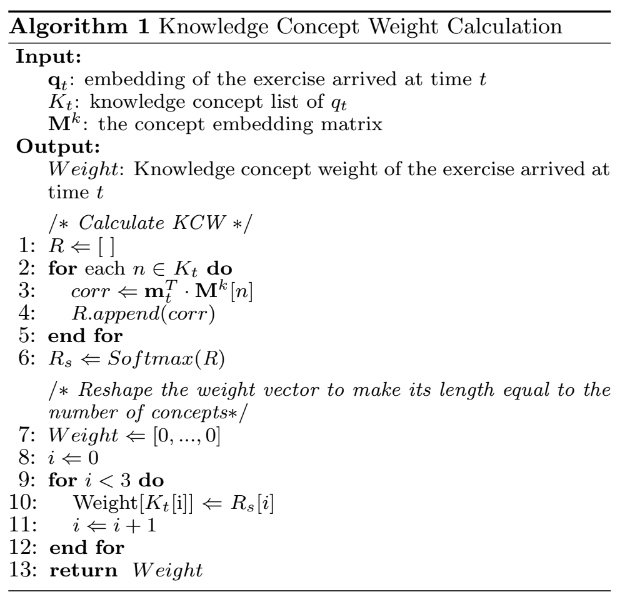
\includegraphics[scale=0.8]{exrec2.png}
	\caption{}
	\label{}
\end{figure}



\subsection{Proces čitanja}


Nakon što se izračunati KCW iskoristi za izračun težinske sume stanja koncepata znanja određenog korisnika $r_t=\sum_{i=1}^{N}w_iM^v_t$, na tu sumu rt se nadodaju značajke težine zadatka i "stage feature" dt,gt. Rezultat se šalje u potpuno povezani sloj sa aktivacijskom funkcijom Tanh kako bi se dobio "summary" vektor koji sadrži sve informacije o studentovom znanju povezanom sa qt i značajkama zadatka.
\begin{equation}
	f_t=Tanh(W_0^T[r_t,d_t,g_t,m_t])
\end{equation}

Na kraju, ft prolazi kroz potpuno povezani sloj koji daje kao izlaz vjerojatnosti da bi student odradio
zadatake qt točno.
\begin{equation}
p=Sigmoid(W^T_1f_t)
\end{equation}


\subsection{Proces ažuriranja}

Proces ažuriranja mijenja vrijednosti matrice $M^v_t$ koja predstavlja trenutno stanje studentovog koncepta znanja \textit{k}.
Ovaj model je drukčiji od DKVMN po tome da se razmatra i trajanje rješavanja. Prema povezanim radovima, trajanje rješavanja zadatka je povezano sa razinom znanja studenta. Pošto je vrijeme rješavanja kontinuirana varijabla ona se prvo diskretizira po njenoj distribuciji i unda se prikaže kao varijabla t te se koristi kako bi se ažurirala matrica $M$. Ostali procesi su isti kao i u DKVMN, sastoji se od podprocessa dodavanja i brisanja. Vektor brisanjas e dobije $e=Sigmoid(E^T[s_t,t])$ dok se vektor dodavanja dobije kao $a=Tanh(D^T[s_t,t])$ te se nova matrica M računa kao
\begin{equation}
	M^v_{t+1}(i+1) =M^v_t (i)[1-w(i)e][1+w(i)]
\end{equation}
Parametri ovog modela se račuaju tako da se minimizira "cross-entropy loss" između pretpostavljenog studentovog
dobvivenog i pretpostavljenog rezultata. 
\begin{equation}
	L=-\sum_t ((y_i \log p_t ) + (1-y_t)\log (1-p_t))
\end{equation}






\section{Preporuka zadataka podržanim učenjem}
\subsection{Općenito o podržanom učenju}
Glavni elementi svakog algoritma podržanog učenja su, osim agenta i okoline, strategija, nagrada, vrijednost (predikcija nagrade) i opcionalno model. Strategija predstavlja agentov način ponašanja u određenom trenutku. Ona je preslikavanje iz spoznatog stanja okoliša u akcije koje je potrebno izvršiti u tim stanjima. Agentova je srž, ona sama je dovoljna da odredi ponašanje. \newline
Cilj podržanog učenja definira nagrada koja preslikava opaženo stanje okoliša (ili par stanje-akcija) u jedan broj koji odgovara poželjnosti tog stanja. Cilj agenta je maksimizirati ukupnu nagradu. Nagrada definira što je trenutno dobro, a funkcija vrijednosti definira što je dugoročno dobro. Vrijednost stanja je očekivanje ukupne količine nagrade koja bi se mogla akumulirati u budućnosti počevši od tog stanja. To očekivanje još se naziva i Q funkcija.\newline
Model imitira ponašanje okoline. Za dano stanje i akciju, model može predvidjeti rezultantno iduće stanje i nagradu.\newline
\newline
U ovom radu okolina se izgrađuje simulatorom temeljenim na DKVMN-CA (CA = \textit{concept aware}). Personalizirani agent za preporučivanje zadataka trenira se dubokim učenjem, točnije korištenjem GRU-a (engl. \textit{Gated Recurrent Unit}): poboljšane verzije standarnih RNN. \newline
\newline
Proces odlučivanja modelira se kao Markovljev proces odlučivanja s djelomično vidljivim stanjima (POMDP).
POMDP je generalizacija Markovljevog procesa odlučivanja. Modelira agentov proces odlučivanja; vezu agenta i okoline.
Formalno, POMDP je skup 7 varijabli (stanje, akcija, uvjetna vjerojatnost prijelaza među stanjima, nagrada, opažanja, uvjetne vjerojatnosti opažanja, koeficijent umanjenja nagrade). Agent u svakom stanju bira akciju koja će maksimizirati buduću nagradu umanjenu za faktor umanjenja.\newline
Osnovna je pretpostavka u podržanom učenju da agent vidi stvarno stanje svijeta. No, agentova opažanja u stvarnom svijetu nisu nužno isto što i pravo stanje: uvodi se vjerojatnost stanja $p(o_i|s_i)$ - vjerojatnost da se za opažanje $o_i$ svijet nalazi u $s_i$. Sljedeće stanje u svijetu ovisi o trenutnom stanju i agentovoj akciji. Dva stanja svijeta mogu rezultirati u jednakom opažanju agenata. Za opažanja ne vrijedi Markovljevo svojstvo (sljedeće opažanje stanja ne ovisi isključivo o trenutnom opažanju i akciji). Potrebno je uzeti u obzir putanju agenta. \newline
\newline
\subsection{Primjena na ExRec}
Konkretno, u ExRec-u stanje modela je studentovo konkretno latentno znanje, a akcija je preporuka zadatka. Strategija preporuka direktno funkcionira na sirovim opažanjima studentove povijesti rješavanja zadataka. U trenutku $t$ agent ne može vidjeti studentovo znanje $s_t$. No, opažanje mu je $o_t$ - zadatak i točnost rješavanja uvjetovani pomoću $s_t$, $p(o_t|s_t)$. Agent preporučuje $a_t$ na temelju povijesti studentovih zadataka $h_t=(o_1, a_1, o_2, a_2, ..., o_{t-1},a_{t-1})$. Nakon završetka preporučenog zadatka, latentno znanje prelazi u $s_{t+1}$ pomoću $p(s_{t+1}|s_t, a_t)$.\newline
Agentu je potrebna strategija kako bi izabrao najbolju akciju za određeno stanje. Nagrada akcije $a_t$ je usrednjena suma vjerojatnosti da će student točno riješiti sljedeći zadatak, $q$, nakon što riješi predloženi zadatak u stanju $s_{t+1}$. Usrednjava se brojem zadataka. Taj sljedeći zadatak predviđen je simulatorom. Algoritam preporučuje zadatak $q$, čija je nagrada maksimalna. Opisano je vidljivo jednadžbom ~\ref{eq:nagr_akc}.\newline
\begin{equation}
r_{t}=\frac{1}{K} \sum_{i=1}^{K} P_{t+1}\left(q_{i}\right)\label{eq:nagr_akc}
\end{equation}
\newline
\newline
Krajnji cilj je maksimizirati nagradu određene strategije gdje su trajektorije $(s_1, o_1, a_1, ...)$ preuzete iz distribucije trajektorija induciranih strategijom $\pi$. Nagrada je izražena jednadžbom ~\ref{eq:nagr_strat}. \newline
\begin{equation}
R=\mathbb{E}_{\tau}\left[\sum_{t=1}^{\infty} \gamma^{t-1} r\left(s_{t}, a_{t}\right)\right]\label{eq:nagr_strat}
\end{equation}
\newline
POMDP se rješava pomoću TRPO algoritma (engl. \textit{Trust Region Policy Optimization}). TRPO je algoritam optimizacije robustan na velik raspon zadataka dajući monotono poboljšanje izmjenom malog broja parametara. Algoritam stalno iznova optimizira lokalne aproksimacije očekivane povratne vrijednosti strategije s kaznom KL-divergencije.\newline
\newline
\section{Evaluacija performansi}
%(ovo ce možda trebati preraditi jer ste mijenjali dataset) izbaciti čak?
Originalni ExRec model evaluiran je na IPS datasetu provodenjem 50 eksperimenata podjelom korisnika na skupove za treniranje i testiranje u omjeru 70:30. Kao mjera performansi odabrana je AUC krivulja. Procjenjena je i efikasnost korištenjem dodatnih značajki modela, poput težine zadataka, faze rješavanja i trajanja rješavanja čija upotreba dokazano poboljšava performanse modela. 
\subsection{Preporuke zadataka}
\subsubsection{Evaluacija porasta znanja studenta}
Algoritmi za treniranje strategije preporuke zadataka pomoću podržanog učenja većinom su heuristički; zadatke ocijenjene kao prelagane ili preteške potrebno je izbjegavati. No, optimalnost takvih algoritama nije zadovoljena jer se u obzir uzima samo kratkoročna nagrada. U ExRec-u se u obzir uzima dugoročna nagrada. \newline
%izbaciti ako nećemo koristiti do kraja?
Kao strategije algoritma podržanog učenja u originalnom ExRec-u korištena su dva algoritma, Expectimax i RL. Kod Expectimaxa prvo se računa iznos predviđenog znanja u slučaju da se preporuči određen zadatak. Sustav kao preporuku izabire zadatak kojim bi maksimizirao predviđeno znanje u tom trenutku. RL razmatra dugoročnu nagradu akcije maksimizacijom Q funkcije.\newline
%(isto izbaciti/izmijeniti ovisno kako cemo mi raditi)
Za usporedbu algoritama, autori rada izvlače 15 studenata iz dataseta. Za oba algoritma inicijaliziraju se simulatori pomoću slijeda prethodno riješenih zadataka svakog studenta. Preporuča se 50 zadataka. Sprema se prosjek predviđenog znanja svih studenata u svakom koraku preporuke. %ubaciti sliku


\subsubsection{Evaluacija preporuka} %izaciti ako nećemo koristiti?
Za proučavanje RL strategije autori su osmislili dodatni eksperiment kojim se uzme student i njegovih prijašnje riješenih 5 zadataka te pokrene simulator. Preporuči mu se novih 5 zadataka pomocu RL. Vizualno se prikaže tih 10 zadataka u obliku (broj zadatka, povezani koncept, točnost). Promatra se povezanost točnosti zadataka i odgovarajućih koncepata. Ako ne postoji znanje o nekom konceptu, grafički prikaz je crne boje. Kako znanje raste, boja je svjetlija.\newline
Kad student netočno riješi zadatak, algoritam mu preporuči povezani koncept. Ako padne i preporučeni zadatak, sustav mu nudi ponovno rješavanje.\newline
Nakon povećanja znanja o nekom konceptu, prebacuje se na neki drugi koncept. Ako je zadatak okarakteriziran kao lagan, znanje se ne povećava pretjerano iako je točno riješen.\newline
Ponovno se preporučuje početni zadatak i stvar se ponavlja dok se ne riješi točno.


\subsection{Rezultati i problemi}
 	\subsubsection{26.8.2020.}
 		Prilagođena je skripta new\_kt kako bi davala parametre za biologiju (smanjen je seq\_len), napravljene su skripte koje stvaraju potrebne .pkl fileove bez da su putevi do datoteka hardkodirani. Također, napravljena je skripta koja dataset dijeli na dio za treniranje i dio za validaciju u formatu koji treba za pokretanje new\_kt.py. Nakon što su broj koncepata i jedinstvenih pitanja postavljeni da odgovaraju datasetu biologije new\_rs.py se može normalno pokrenuti.
\newline
Za razliku od assistmentsa vrijednosti porasta znanja u svakom koraku su oko 0.507 te slabo osciliraju.
 		\begin{figure}[!htb]
 			\centering
 			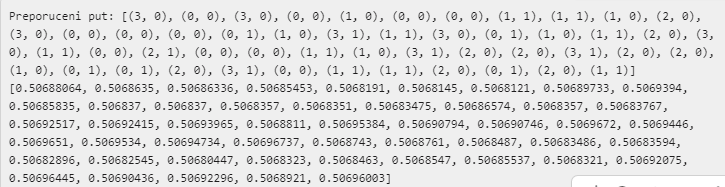
\includegraphics[scale=0.8]{exrec_bio1.png}
 			\caption{}
 			\label{}
 		\end{figure}
 	
 	\begin{figure}[!htb]
 		\centering
 		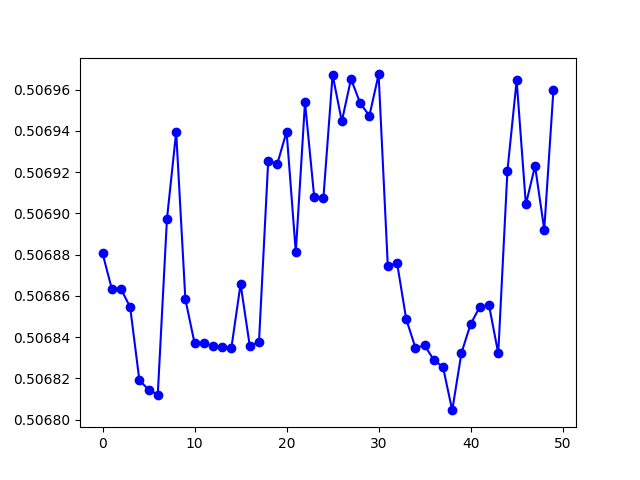
\includegraphics[scale=0.8]{exrec_bio2.png}
 		\caption{}
 		\label{}
 	\end{figure}
 		
 	I dalje nije jasno koje vrijednosti hiperparametara poput seq\_len i veličina memorije bi se trebali koristiti te koje je pravo značenje "porasta/vrijednosti" znanja u svakom trenutku. Za iste parametre i dataset new\_rs.py uvijek daje drugačiji put preporuke što nije poželjno. Potrebno je i omogućiti izvedbu RS-a po chunkovima Assistmentsa koji nisu hardkodirani. Iz nekog razloga kada se koristi biologija trebaju se zakomentirati sve "isnan" funkcije, dok su iste potrebne kod assitmentsa.

\section{Poveznice}
\url{http://incompleteideas.net/book/first/ebook/node9.html}
\url{https://towardsdatascience.com/understanding-gru-networks-2ef37df6c9be}
\url{https://en.wikipedia.org/wiki/Partially_observable_Markov_decision_process}
\url{https://medium.com/@jonathan_hui/rl-trust-region-policy-optimization-trpo-explained-a6ee04eeeee9}
\url{https://arxiv.org/abs/1502.05477}

